\section{Resultados}


Simulamos os dois modelos para diferentes condições iniciais e valores de parâmetros.
Utilizamos o software \emph{SageMath 9.0} para realizar as simulações.
Resolvemos todos os sistemas utilizando o algoritmo Runge-Kutta-Prince-Dormand 8-9.
Os valores padrão de parâmetros utilizados nas simulações se encontram na Tabela \ref{tab: params}.

\begin{table}[ht!]
    \begin{center}
        \begin{tabular}{l l}
            \hline
            \emph{Parâmetros e constantes} & \emph{Valores} \\
            \hline
            \( \mu_{ T } \): taxa de mortalidade de células T CD4+ não infectadas & 0.01 \unit{dia^{ -1 }} \\
            \( \mu_{ T_{ i } } \): taxa de mortalidade de células T CD4+ infectadas & 0.5 \unit{dia^{ -1 }} \\
            \( k_{ s } \): taxa de células T CD4+ infectadas por vírus suscetível & \( 2.3233 \cdot 10^{ -4 } \) \unit{mm^{ 3 } dia^{ -1 }} \\
            \( k_{ r } \): taxa de células T CD4+ infectadas por vírus resistente & \( 2.32 \cdot 10^{ -4 } \) \unit{mm^{ 3 } dia^{ -1 }} \\
           \( k_{ \nu } \): taxa com a qual células T CD4+ matam o vírus & 0.00825 \unit{mm^{ 3 } dia^{ -1 }} \\
           \( p \): taxa de proliferação de células T CD4+ não infectadas & 0.05 \unit{dia^{ -1 }} \\
           \( p_{ i } \): taxa de proliferação de células T CD4+ infectadas & 0.05 \unit{dia^{ -1 }} \\
           \( G_{ s } \): taxa de entrada de vírus sensíveis no sangue & 330 \unit{mm^{ -3 } dia^{ -1 }} \\
           \( G_{ r } \): taxa de entrada de vírus resistentes no sangue & \( 0.9995 \cdot G_{ s } \) \unit{mm^{ -3 } dia^{ -1 }} \\
           \( q \): probabilidade de mutação do vírus & 0.999 \\
           \( N \): número de partículas virais viáveis geradas na lise & 10 \\
           \( C \): constante de meia-saturação de células T CD4+ não infectadas & 188 \unit{mm^{ -3 }} \\
           \( C_{ i } \): constante de meia-saturação de células T CD4+ infectadas & 188 \unit{mm^{ -3 }} \\
           \( B \): constante de meia saturação da entrada de vírus externo. & \( 12 \) \unit{mm^{ -3 }} \\
           \( B_{ s } \): constante de meia saturação da fonte de céulas T CD4+ & \( 55 \) \unit{mm^{ -3 }} \\
           \( \mu \): parâmetro de tratamento & 0.9 \\
           \( \eta \): parâmetro de tratamento & 0.15 \\
           \( \rho \): parâmetro de tratamento & 0.05 \\
           \hline
        \end{tabular}
        \caption{Valores padrão de parâmetros para os modelos com e sem tratamento.}
        \label{tab: params}
    \end{center}
\end{table}

\subsection{Sem tratamento}

Como mencionado na seção anterior, o parâmetro \( G_{ s } \) dita como ocorre o percurso da doença.
Portanto, realizamos três simulações com diferentes valores para esse parâmetro e em cada uma obtivemos um equilíbrio distinto, correspondentes a três possíveis desenvolvimentos da infecção.
Os resultados das simulações estão na Figura \ref{fig: no_treat_scenarios}.
Em todos eles, as populações iniciais tomadas foram \( T ( 0 ) = 1000, V_{ s } ( 0 ) = 10 \) e \( T_{ s } ( 0 ) = 0 \).

\begin{figure}[ht!]
    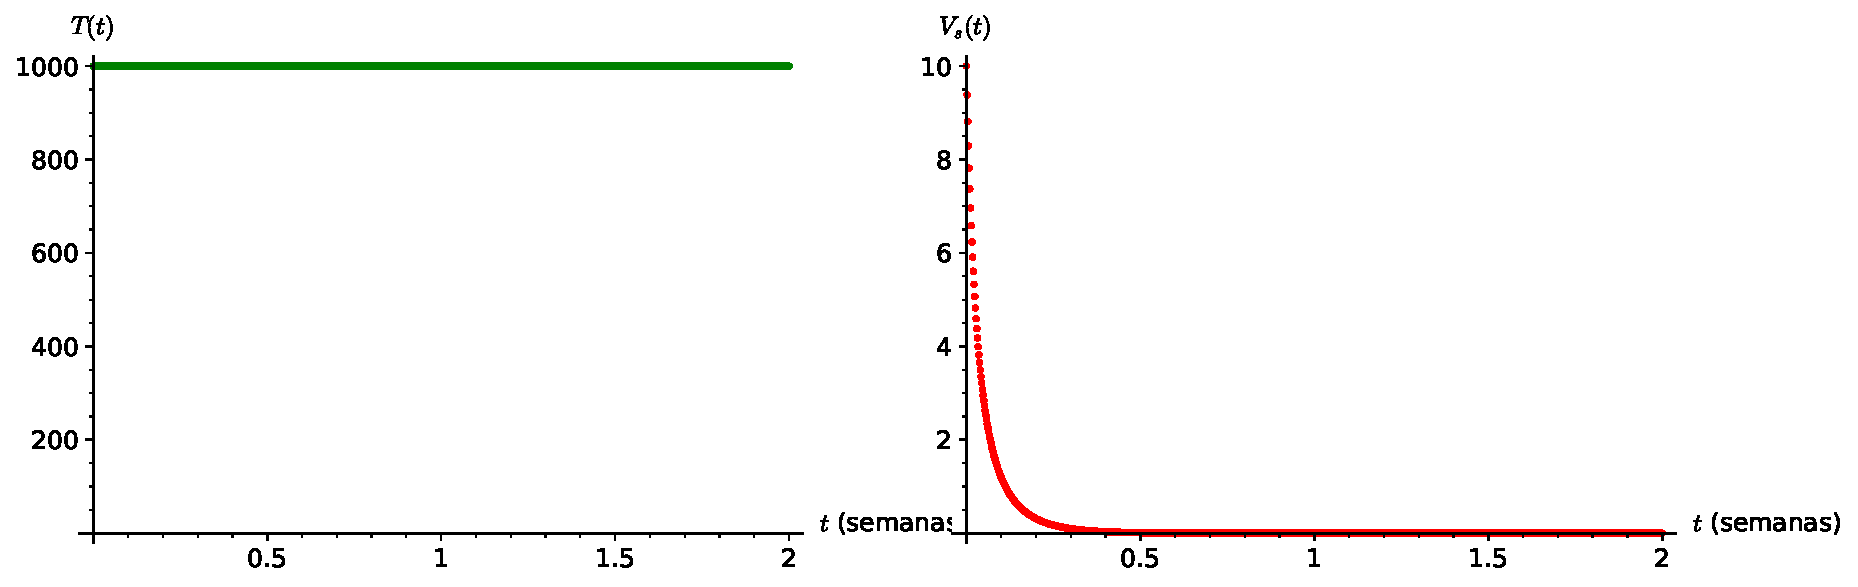
\includegraphics[width=\textwidth]{figuras/cenario_1.pdf}
    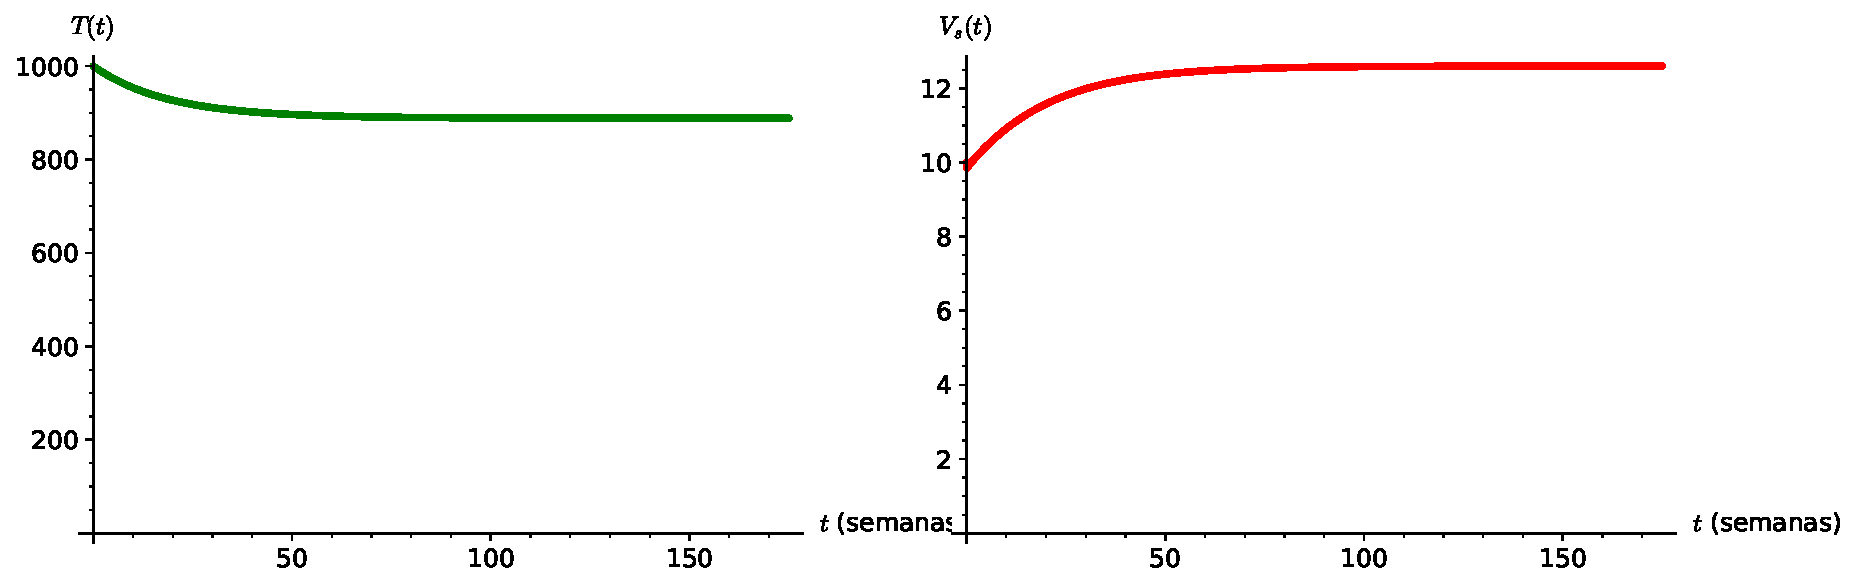
\includegraphics[width=\textwidth]{figuras/cenario_2.pdf}
    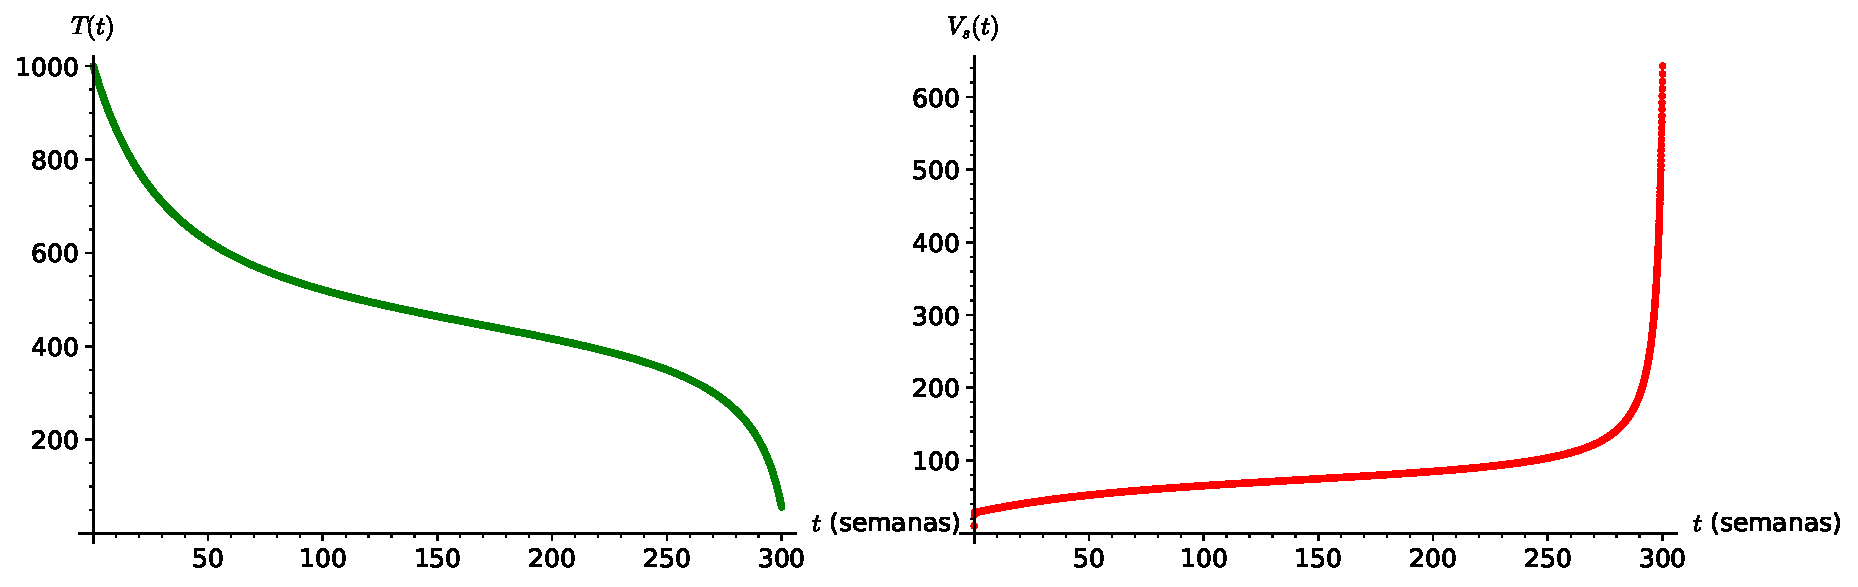
\includegraphics[width=\textwidth]{figuras/cenario_3.pdf}
    \caption{Evolução das populações de células T saudáveis e de vírus, no cenário sem tratamento.
    De cima para baixo, os valores utilizados para \( G_{ s } \) em cada simulação são: 80, 180, 330.}
    \label{fig: no_treat_scenarios}
\end{figure}

\subsection{Com tratamento}

Nas simulações com tratamento combinado tomamos \( G_{ s } = 330 \).
O tempo \( t_{ 0 } \) é definido como o tempo em que a população de células \( T \) saudáveis atinge um nível pré-fixado.
Na Figura \ref{fig: treat_both_pops}, vemos a evolução típica da infecção no modelo com tratamento combinado.
Simulamos três cenários, nos quais o tratamento começa assim que a população de células T atinge os valores de \( 200, 300 \) e \( 500 \) indivíduos por \unit{mm^{ 3 }}, respectivamente.
Em todos eles, a variante resistente do vírus apareceu \( t_{ r } = 30 \) semanas após o início do tratamento.
Vemos que, independentemente de quando o tratamento começa, eventualmente a população de células T é extinta.

\begin{figure}[ht!]
    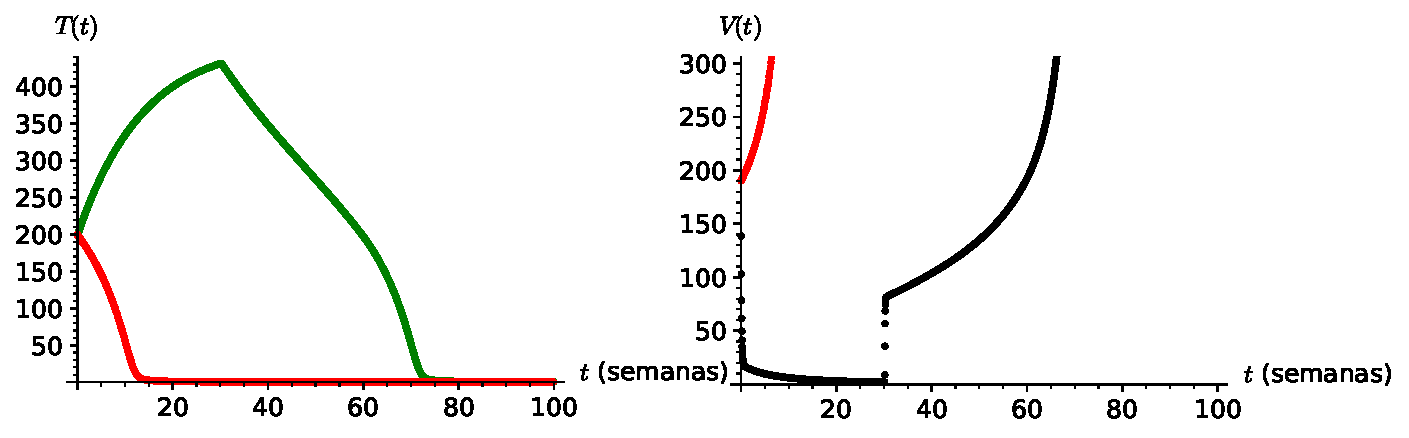
\includegraphics[width=\textwidth]{./figuras/start_treatment_at_T_200.pdf}
    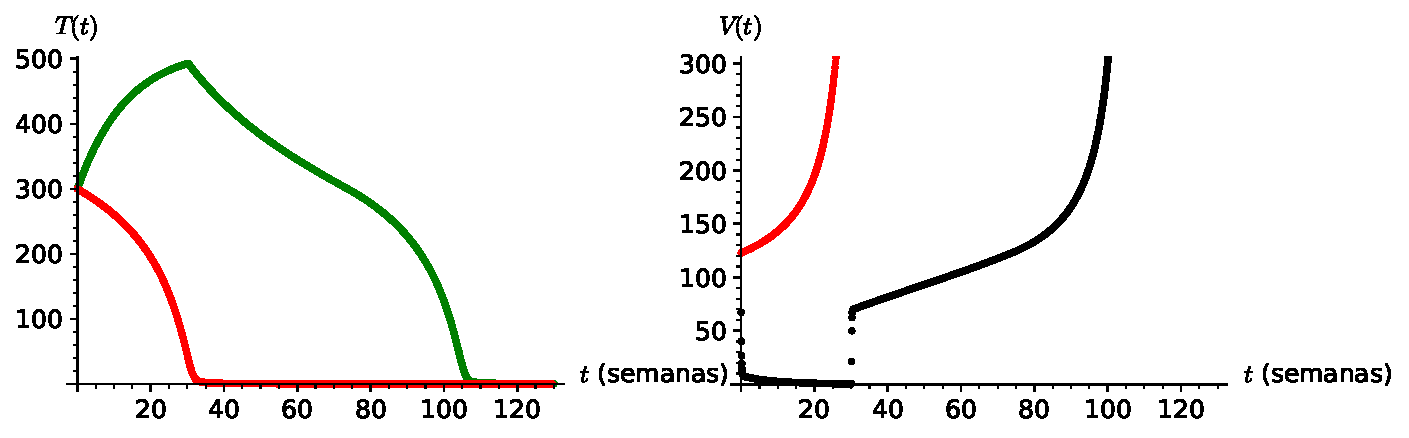
\includegraphics[width=\textwidth]{./figuras/start_treatment_at_T_300.pdf}
    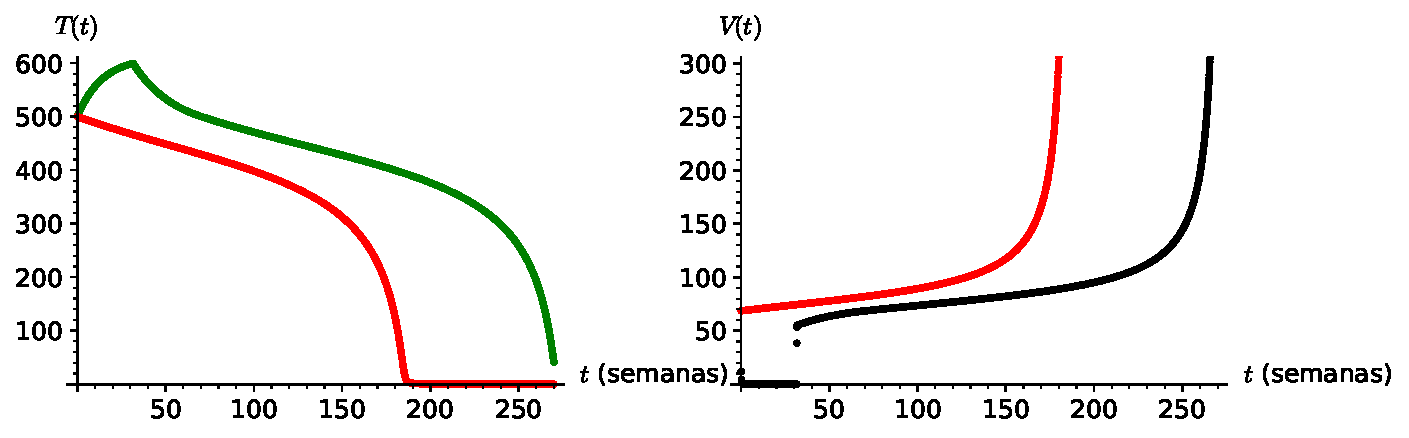
\includegraphics[width=\textwidth]{./figuras/start_treatment_at_T_500.pdf}
    \caption{ Evolução das populações \( T ( t ) \) de células T e \( V ( t ) = V_{ s } ( t ) + V_{ r } ( t ) \) de vírus a partir do início do tratamento.
    De cima para baixo, o tratamento foi iniciado quando a população de células T atingiu as marcas de \( 200, 300 \) e 500 indivíduos por \unit{mm^{ 3 }}, respectivamente.
    Em todas as simulações, consideramos que a variante viral resistente apareceu \( t_{ r } = 30 \) semanas após o início do tratamento.
    Em todos os gráficos, as linhas vermelhas representam a evolução da população sem tratamento.}
    \label{fig: treat_both_pops}
\end{figure}

Na Figura \ref{fig: multiple_starts_tr30} juntamos as simulações para a evolução da infecção quando o tratamento é iniciado em diferentes patamares da população de células T CD4+.
Nessas simulações, mantivemos \( t_{ r } = 30 \) semanas.
Nas Figuras \ref{fig: multiple_starts_tr20} e \ref{fig: multiple_starts_tr40} repetimos o mesmo experimento, porém alterando o valor de \( t_{ r } \) para \( 20 \) e \( 40 \) semanas, respectivamente.
Nas três figuras \ref{fig: multiple_starts_tr30}, \ref{fig: multiple_starts_tr20} e \ref{fig: multiple_starts_tr40}, percebe-se que o tratamento que resultou na maior longevidade foi o que começou quando a população de células \( T \) atingiu \( 400 \) indivíduos por \unit{mm^{ 3 }} no sangue.

\begin{figure}[ht!]
    \begin{center}
        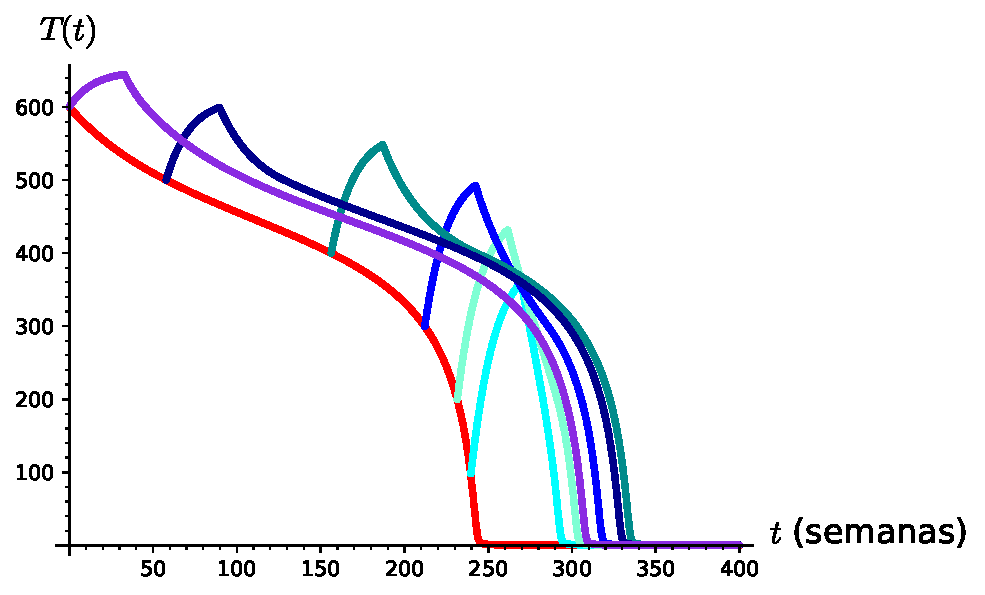
\includegraphics[width=.85\textwidth]{./figuras/different_start_tr210.pdf}
    \end{center}
    \caption{Evolução da população \( T ( t ) \) de células T CD4+ quando o tratamento começa assim que \( T \) atinge os valores de \( 600, 500, 400, 300, 200 \) e \( 100 \) indivíduos por \unit{mm^{ 3 }}, respectivamente.
    A curva vermelha é a evolução sem tratamento.
    Aqui consideramos \( t_{ r } = 30 \) semanas após o início do tratamento.}
    \label{fig: multiple_starts_tr30}
\end{figure}

\begin{figure}[ht!]
    \begin{center}
        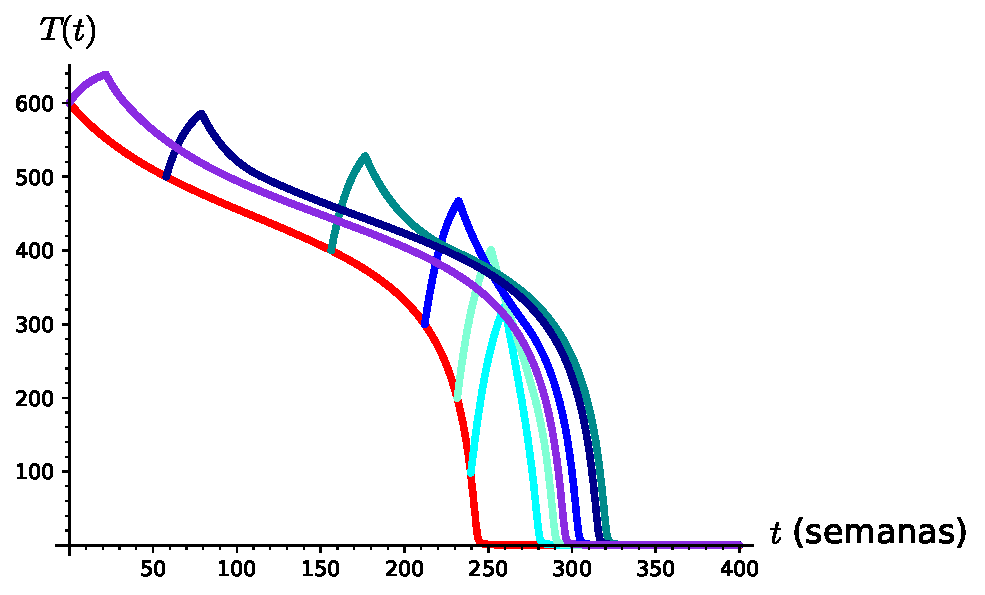
\includegraphics[width=.85\textwidth]{./figuras/different_start_tr140.pdf}
    \end{center}
    \caption{Evolução da população \( T ( t ) \) de células T CD4+ quando o tratamento começa assim que \( T \) atinge os valores de \( 600, 500, 400, 300, 200 \) e \( 100 \) indivíduos por \unit{mm^{ 3 }}, respectivamente.
    A curva vermelha é a evolução sem tratamento.
    Aqui consideramos \( t_{ r } = 20 \) semanas após o início do tratamento.}
    \label{fig: multiple_starts_tr20}
\end{figure}

\begin{figure}[ht!]
    \begin{center}
        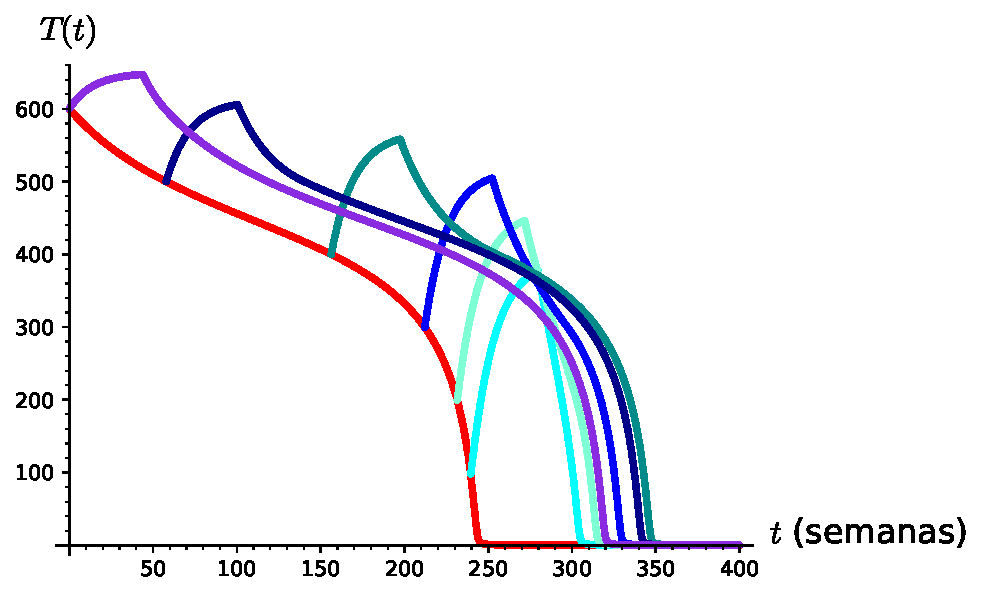
\includegraphics[width=.85\textwidth]{./figuras/different_start_tr280.pdf}
    \end{center}
    \caption{Evolução da população \( T ( t ) \) de células T CD4+ quando o tratamento começa assim que \( T \) atinge os valores de \( 600, 500, 400, 300, 200 \) e \( 100 \) indivíduos por \unit{mm^{ 3 }}, respectivamente.
    A curva vermelha é a evolução sem tratamento.
    Aqui consideramos \( t_{ r } = 40 \) semanas após o início do tratamento.}
    \label{fig: multiple_starts_tr40}
\end{figure}



%% Discussao

% Quando \( G_{ s } = 80 \), percebemos que a população de células \( T \) permanece inalterada e a população viral rapidamente se extingue.
% Porém, aumentando o valor de \( G_{ s } \) para \( 180 \), percebemos uma mudança 
